\begin{figure}
  \centering

  \begin{minipage}{.65\textwidth}
    \centering
    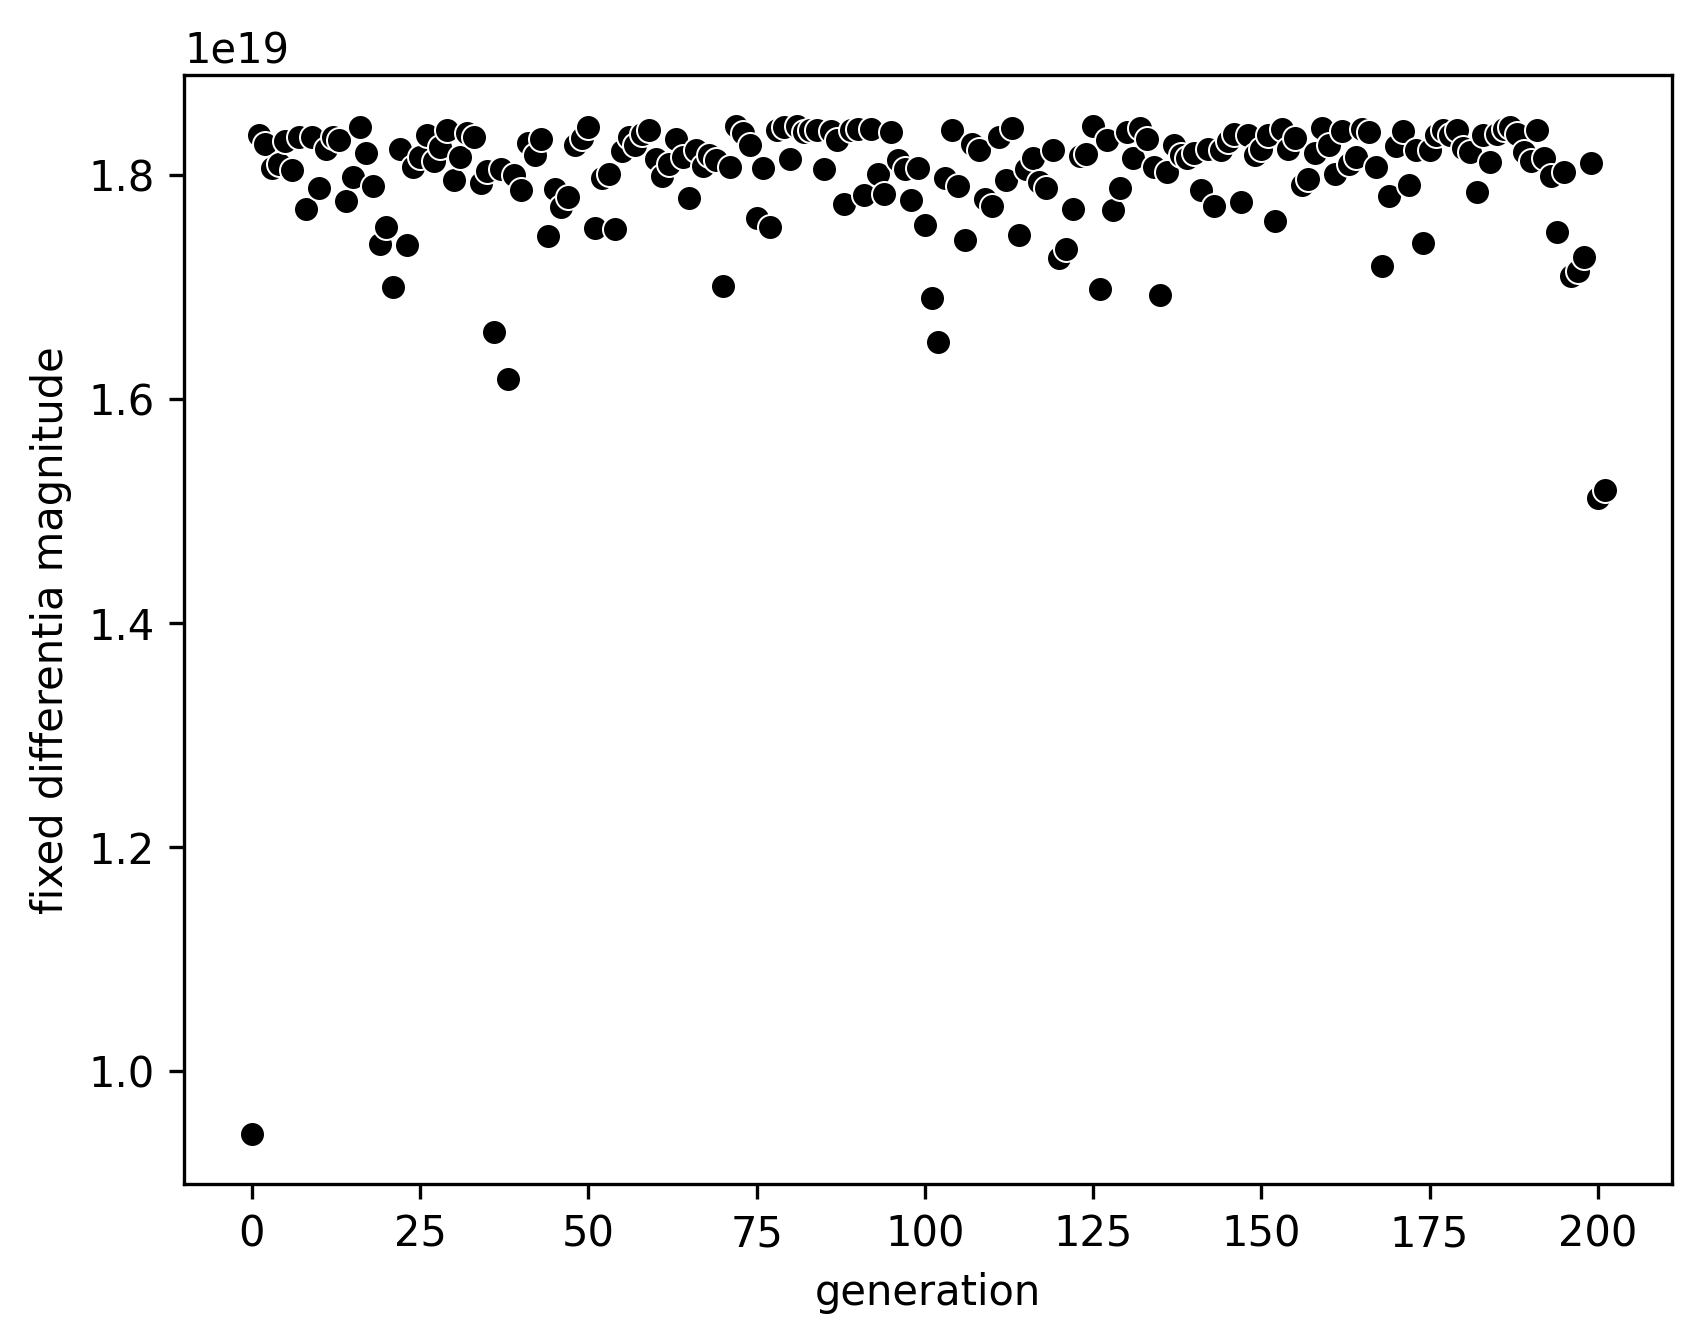
\includegraphics[height=0.25\textheight]{notebooks/notebooks/teeplots/notebook=ne-inference+replicate=0+treatment=control+viz=scatterplot-differentia-magnitude+ext=}
  \end{minipage}%
  \begin{minipage}{.25\textwidth}
    \subcaption{Fixed Species-level Differentia Magnitudes by Layer}
    \label{fig:ne-process-example:differentia}
  \end{minipage}

  \vspace{0.25em}

  \begin{minipage}{.65\textwidth}
    \centering
    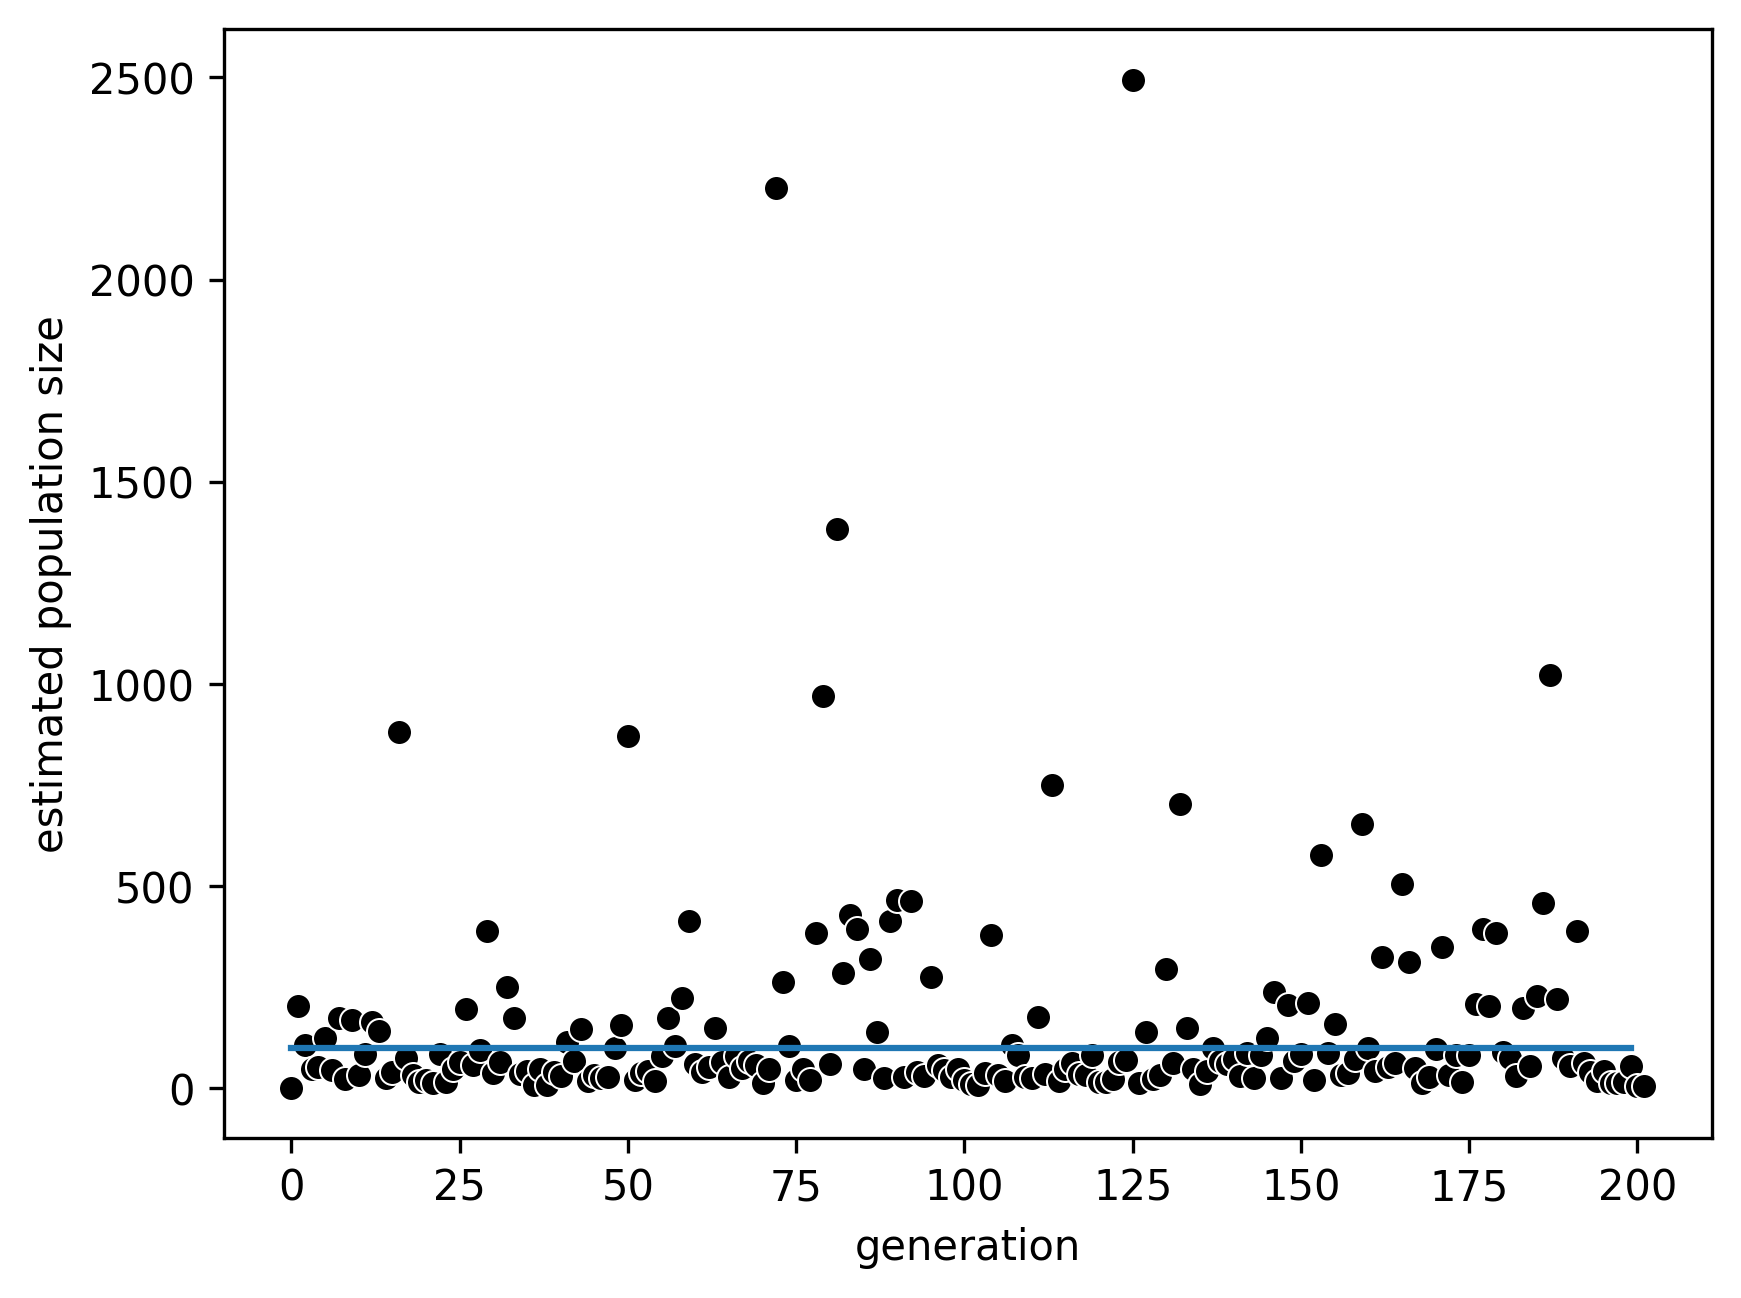
\includegraphics[height=0.25\textheight]{notebooks/notebooks/teeplots/notebook=ne-inference+replicate=0+treatment=control+viz=scatterplot-popsize-estimates+ext=}
  \end{minipage}%
  \begin{minipage}{.25\textwidth}
    \subcaption{Population Size Estimates}
    \label{fig:ne-process-example:singleton-est}
  \end{minipage}

  \vspace{0.25em}

  \begin{minipage}{.65\textwidth}
    \centering
    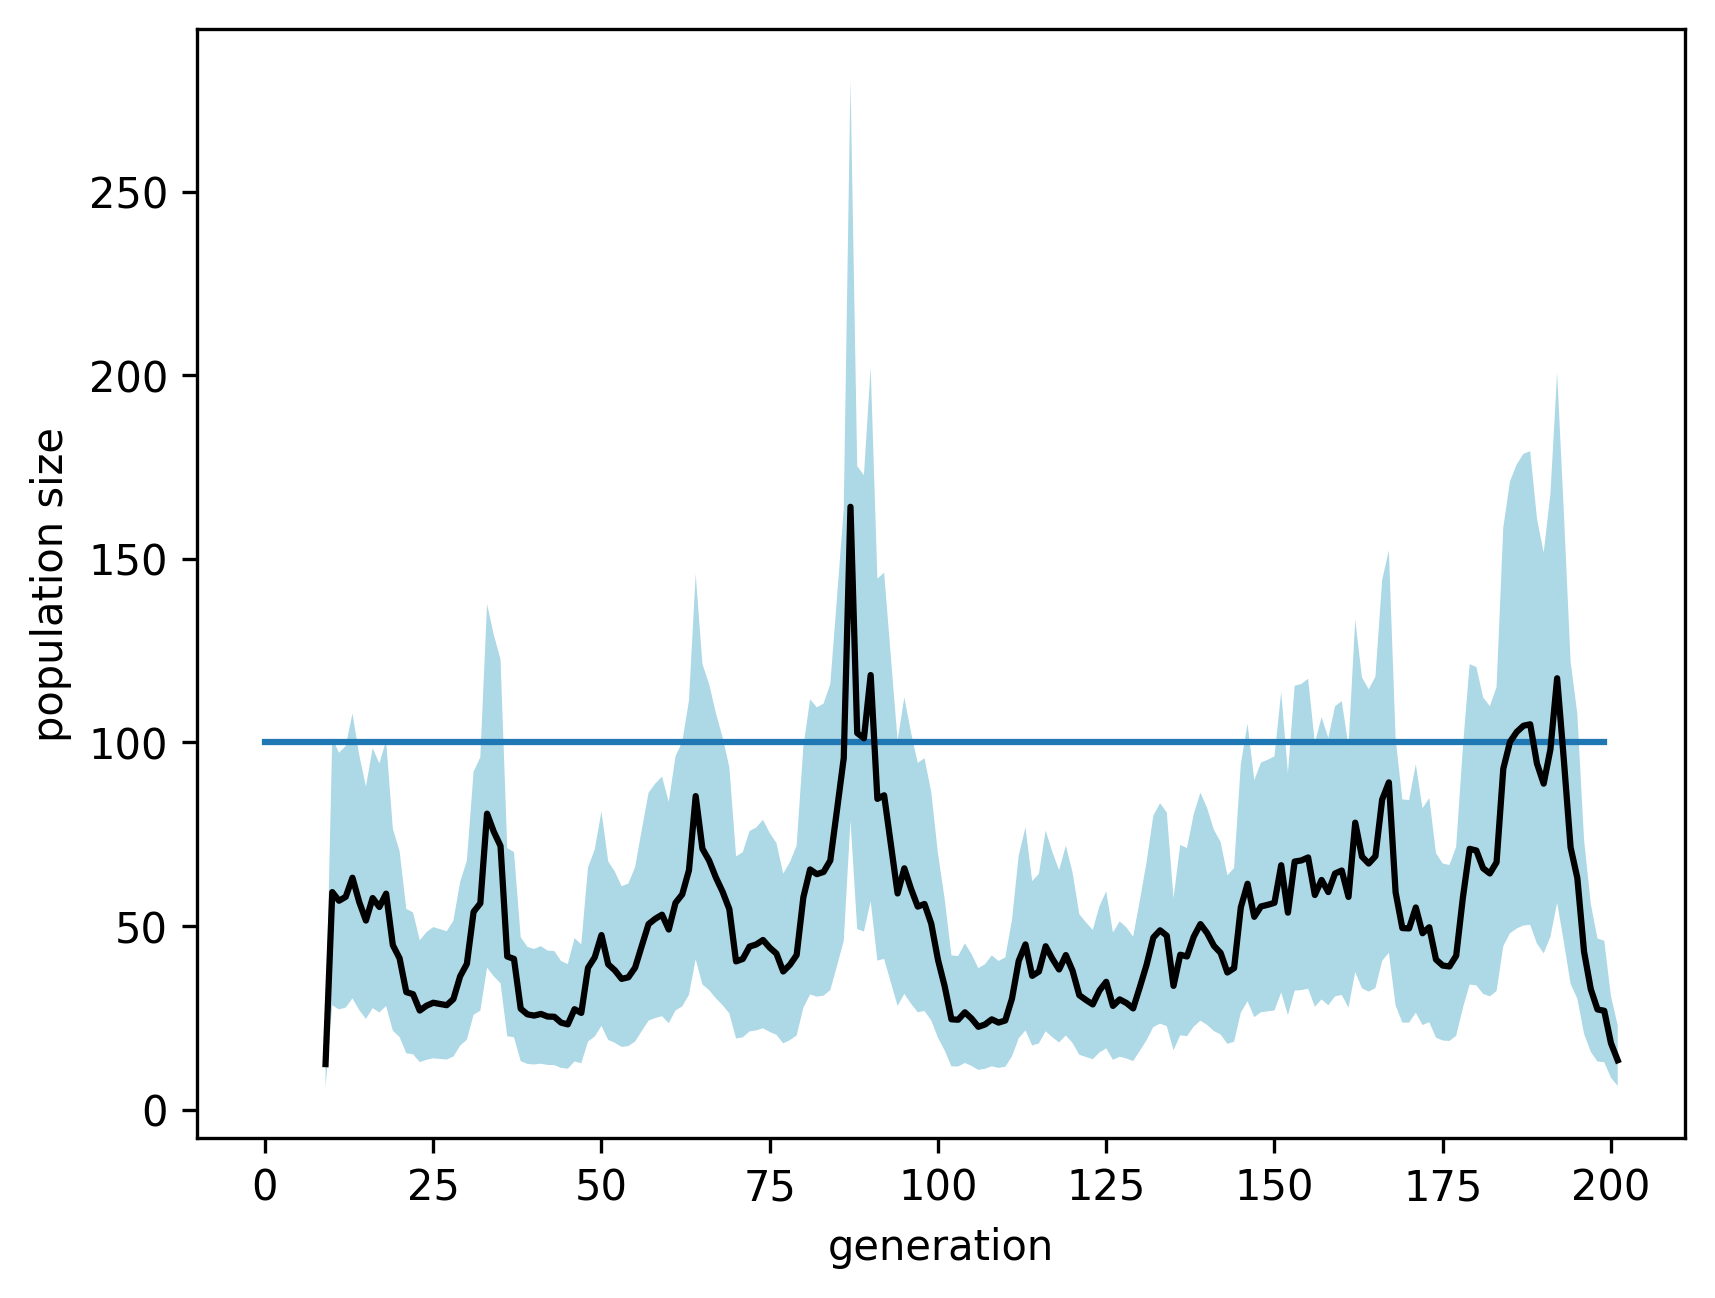
\includegraphics[height=0.25\textheight]{notebooks/notebooks/teeplots/notebook=ne-inference+replicate=0+treatment=control+viz=plot-running-estimation+x=rank+y=population-size+ext=}
  \end{minipage}%
  \begin{minipage}{.25\textwidth}
    \subcaption{Running Population Size Estimation with 95\% Confidence Intervals}
    \label{fig:ne-process-example:running-est}
  \end{minipage}

  \caption{
    Example population size estimation data.
    Differentia values are extracted from species-level annotation of a single extant population member (Subfigure \ref{fig:ne-process-example:differentia}).
    Subfigure \ref{fig:ne-process-example:singleton-est} shows one-off population size estimates at each generation from the corresponding differentia.
    To improve statistical informativeness, differentia values are grouped into a running pool of ten values to perform population size estimation.
    True population carrying capacity is annotated as a horizontal line.
    Note that systematic underestimation of ``carrying capacity'' population size is expected due to demographic factors excluding some population members from gene pool contributions.
    Figure \ref{fig:beta-explain} overviews the statistical mechanism used for population size distribution.
  }
  \label{fig:ne-process-example}
\end{figure}


% notebooks/notebooks/teeplots/notebook=ne-inference+replicate=0+treatment=control+viz=plot-running-estimation+x=rank+y=population-size+ext=.pdf
%
% notebooks/notebooks/teeplots/notebook=ne-inference+replicate=0+treatment=control+viz=scatterplot-differentia-magnitude+ext=.pdf
%
% notebooks/notebooks/teeplots/notebook=ne-inference+replicate=0+treatment=control+viz=scatterplot-popsize-estimates+ext=.pdf


% notebooks/notebooks/teeplots/notebook=ne-inference+replicate=0+treatment=bottleneck+viz=plot-running-estimation+x=rank+y=population-size+ext=.pdf
%
% notebooks/notebooks/teeplots/notebook=ne-inference+replicate=0+treatment=bottleneck+viz=scatterplot-differentia-magnitude+ext=.pdf
%
% notebooks/notebooks/teeplots/notebook=ne-inference+replicate=0+treatment=bottleneck+viz=scatterplot-popsize-estimates+ext=.pdf

% notebooks/notebooks/teeplots/notebook=ne-inference+replicate=0+treatment=range-expansion+viz=plot-running-estimation+x=rank+y=population-size+ext=.pdf
%
% notebooks/notebooks/teeplots/notebook=ne-inference+replicate=0+treatment=range-expansion+viz=scatterplot-differentia-magnitude+ext=.pdf
%
% notebooks/notebooks/teeplots/notebook=ne-inference+replicate=0+treatment=range-expansion+viz=scatterplot-differentia-magnitude+ext=.pdf
%
% notebooks/notebooks/teeplots/notebook=ne-inference+replicate=0+treatment=selection-pressure+viz=plot-running-estimation+x=rank+y=population-size+ext=.pdf
%
% notebooks/notebooks/teeplots/notebook=ne-inference+replicate=0+treatment=selection-pressure+viz=scatterplot-differentia-magnitude+ext=.pdf
%
% notebooks/notebooks/teeplots/notebook=ne-inference+replicate=0+treatment=selection-pressure+viz=scatterplot-popsize-estimates+ext=.pdf
